% Method overview figure (TikZ). Needs: \usepackage{tikz},
% \usetikzlibrary{arrows.meta,positioning,shapes.geometric,calc,patterns}
% and the thumbnails in figures/: test_image.png, gt_mask.png,
% map_routeA.png, ref1.png ... ref4.png
\definecolor{ink}{HTML}{1F2A44}
\definecolor{slateA}{HTML}{6E7D99}
\definecolor{tealB}{HTML}{0F9E8E}
\definecolor{amberF}{HTML}{D98E04}
\definecolor{crim}{HTML}{D1366B}
\definecolor{panel}{HTML}{F3F5F9}
\begin{tikzpicture}[x=1cm,y=1cm, font=\sffamily\scriptsize, ink,
  arr/.style={-{Latex[length=1.6mm,width=1.3mm]}, line width=0.6pt, ink},
  lane/.style={rounded corners=3pt, line width=0.6pt},
  stage/.style={rounded corners=5pt, fill=panel, draw=none},
  head/.style={font=\sffamily\footnotesize\bfseries, anchor=north west},
  op/.style={circle, draw=ink, line width=0.6pt, fill=white, inner sep=1pt, minimum size=5.2mm, font=\sffamily\tiny\bfseries},
  thumb/.style={inner sep=0pt, draw=ink, line width=0.4pt}]

% ---------------- stage backgrounds ----------------
\fill[stage] (0,0) rectangle (3.95,6.0);
\fill[stage] (4.1,0) rectangle (12.95,6.0);
\fill[stage] (13.1,0) rectangle (18.0,6.0);
\node[head] at (0.12,5.92) {(a) Frozen features};
\node[head] at (4.22,5.92) {(b) Score each patch against a reference};
\node[head] at (13.22,5.92) {(c) Evaluation and analysis};

% ---------------- (a) features ----------------
\node[thumb] (img) at (0.95,3.55) {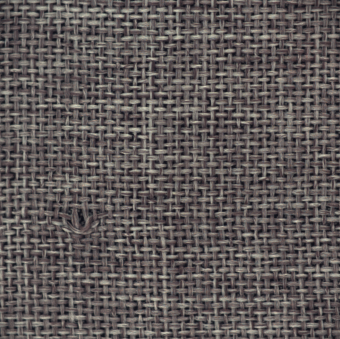
\includegraphics[width=1.55cm]{test_image.png}};
\foreach \k in {1,...,6} {
  \draw[white, opacity=0.55, line width=0.25pt] ($(img.south west)+(\k*1.55/7,0)$) -- ++(0,1.55);
  \draw[white, opacity=0.55, line width=0.25pt] ($(img.south west)+(0,\k*1.55/7)$) -- ++(1.55,0);
}
\node[align=center, below=1pt of img] (imglab) {Test image\\$518\times518$ px};
\fill[tealB!15, draw=ink, line width=0.6pt] (1.95,2.75) -- (2.7,3.1) -- (2.7,4.0) -- (1.95,4.35) -- cycle;
\node[align=center, font=\sffamily\tiny\bfseries] at (2.32,3.55) {DINOv2\\ViT-B/14};
\node[font=\sffamily\tiny, text=tealB!70!black] at (2.32,2.55) {frozen};
\draw[arr] (img.east) -- (1.95,3.55);
\foreach \d in {2,1,0} {
  \foreach \i in {0,...,3} \foreach \j in {0,...,3} {
    \fill[draw=white, line width=0.3pt, fill=tealB!\fpeval{25+10*\d}] ($(2.92,3.05)+(\i*0.19+\d*0.07,\j*0.19+\d*0.07)$) rectangle ++(0.19,0.19);
  }
}
\draw[arr] (2.7,3.55) -- (2.9,3.55);
\node[align=center] at (3.35,2.55) {1,369 tokens\\768-d};

% ---------------- (b) three lanes ----------------
% Route A lane
\draw[lane, fill=slateA!12, draw=slateA] (4.25,4.05) rectangle (11.15,5.45);
\node[anchor=north west, font=\sffamily\scriptsize\bfseries, text=slateA!80!black] at (4.32,5.42) {Route A \,|\, mean self-similarity};
\node[anchor=north east, font=\sffamily\tiny\itshape, text=crim] at (11.1,5.4) {a large defect enters the mean};
\foreach \i in {0,...,4} \foreach \j in {0,...,4} {
  \pgfmathsetmacro{\isdef}{(\i>=1 && \i<=2 && \j<=1) ? 1 : 0}
  \ifdim\isdef pt>0.5pt
    \fill[crim, draw=white, line width=0.3pt] ($(4.45,4.25)+(\i*0.15,\j*0.15)$) rectangle ++(0.15,0.15);
  \else
    \fill[slateA!45, draw=white, line width=0.3pt] ($(4.45,4.25)+(\i*0.15,\j*0.15)$) rectangle ++(0.15,0.15);
  \fi
}
\node[anchor=west, align=left, font=\sffamily\tiny] at (5.25,4.6) {reference: all $N$ patches\\of the \textbf{same} image};
\node[op] (opA) at (7.6,4.6) {mean};
\draw[arr] (7.1,4.6) -- (opA);
\node[anchor=west] at (7.92,4.6) {$s_A(i)=1-\tfrac{1}{N}\sum_{j} \cos(\mathbf{x}_i,\mathbf{x}_j)$};

% Route B lane
\draw[lane, fill=tealB!10, draw=tealB] (4.25,2.1) rectangle (11.15,3.75);
\node[anchor=north west, font=\sffamily\scriptsize\bfseries, text=tealB!75!black] at (4.32,3.72) {Route B \,|\, few-shot memory bank};
\node[anchor=south east, font=\sffamily\tiny\itshape, text=tealB!75!black] at (11.1,2.16) {reference from other images};
\node[thumb] (r1) at (4.86,3.06) {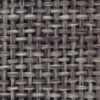
\includegraphics[width=0.34cm]{ref1.png}};
\node[thumb, right=0.04cm of r1] (r2) {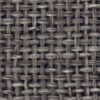
\includegraphics[width=0.34cm]{ref2.png}};
\node[thumb, below=0.04cm of r1] (r3) {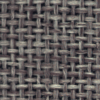
\includegraphics[width=0.34cm]{ref3.png}};
\node[thumb, below=0.04cm of r2] (r4) {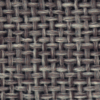
\includegraphics[width=0.34cm]{ref4.png}};
\node[font=\sffamily\tiny, anchor=north] at (5.06,2.51) {$K{=}4$ clean images};
\node[cylinder, shape border rotate=90, aspect=0.25, draw=ink, line width=0.6pt, fill=tealB!25,
      minimum width=0.78cm, minimum height=0.7cm, align=center, font=\sffamily\tiny] (bank) at (6.2,2.82) {5,476\\patches};
\draw[arr] (5.33,2.84) -- (5.8,2.82);
\draw[arr] (6.6,2.83) -- (7.18,2.85);
\node[op] (opB) at (7.45,2.85) {max};
\node[anchor=west] at (7.74,2.85) {$s_B(i)=1-\max_{\mathbf{m}\in\mathcal{M}} \cos(\mathbf{x}_i,\mathbf{m})$};

% FCA lane
\draw[lane, fill=amberF!10, draw=amberF] (4.25,0.2) rectangle (11.15,1.95);
\node[anchor=north west, font=\sffamily\scriptsize\bfseries, text=amberF!85!black] at (4.32,1.92) {Published single-image references};
\node[anchor=north west, align=left] at (4.38,1.5) {\textbf{FCA} (official code): median reference, WideResNet-50\\[1pt]\textbf{Aota-style} (same repository): $K{=}400$, $320\times320$ px\\[1pt]\textit{FCA reproduction checked against its published results}};

% arrows from tokens and from the image
\draw[arr] (3.85,3.95) .. controls (4.05,4.55) .. (4.25,4.6);
\draw[arr] (3.85,3.25) .. controls (4.05,2.9) .. (4.25,2.85);
\draw[arr] (imglab.south) |- (4.25,1.05);

% anomaly map
\node[thumb] (map) at (12.05,3.4) {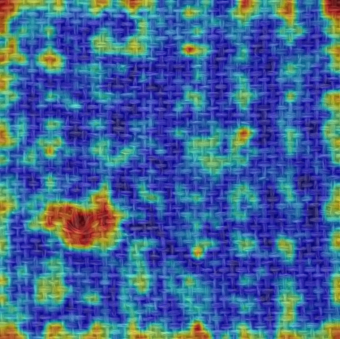
\includegraphics[width=1.3cm]{map_routeA.png}};
\node[align=center, below=1pt of map, font=\sffamily\tiny] {anomaly map\\upsample + $15{\times}15$\\Gaussian ($\sigma\approx2.6$)};
\draw[arr] (11.15,4.75) -- (11.3,4.75) |- ($(map.west)+(0,0.35)$);
\draw[arr] (11.15,2.85) -- (11.3,2.85) |- ($(map.west)+(0,-0.05)$);
\draw[arr] (11.15,1.05) -- (11.3,1.05) |- ($(map.west)+(0,-0.45)$);

% ---------------- (c) analysis ----------------
% metrics
\draw[lane, fill=white, draw=ink!40] (13.25,4.05) rectangle (17.85,5.45);
\node[anchor=north west, font=\sffamily\scriptsize\bfseries] at (13.32,5.42) {1. Metrics on 515 test images};
\draw[line width=0.6pt] (13.45,4.2) rectangle ++(0.55,0.55);
\fill[pattern=north east lines, pattern color=ink!50] (14.2,4.2) rectangle ++(0.55,0.55);
\fill[white] (14.27,4.27) rectangle ++(0.41,0.41);
\draw[line width=0.6pt] (14.2,4.2) rectangle ++(0.55,0.55);
\node[anchor=west, align=left] at (14.9,4.55) {Pixel AP, AU-PRO,\\pixel and image AUROC};
\node[font=\sffamily\tiny, align=center] at (14.15,4.95) {full \;/\; border ignored};

% size analysis
\draw[lane, fill=white, draw=ink!40] (13.25,2.25) rectangle (17.85,3.75);
\node[anchor=north west, font=\sffamily\scriptsize\bfseries] at (13.32,3.72) {2. Size analysis (382 defective images)};
\begin{scope}[shift={(13.55,2.4)}, xscale=0.8]
  \draw[-{Latex[length=1mm]}, line width=0.5pt] (0,0) -- (1.45,0);
  \draw[-{Latex[length=1mm]}, line width=0.5pt] (0,0) -- (0,0.95);
  \node[font=\sffamily\tiny, anchor=north] at (0.75,0.0) {};
  \foreach \px/\py in {0.15/0.88,0.3/0.8,0.42/0.84,0.55/0.7,0.7/0.66,0.85/0.55,1.0/0.5,1.15/0.38,1.3/0.3}
     \fill[slateA] (\px,\py) circle (0.025);
  \foreach \px/\py in {0.15/0.86,0.32/0.86,0.45/0.82,0.6/0.82,0.75/0.79,0.9/0.76,1.05/0.77,1.2/0.72,1.32/0.7}
     \fill[tealB] (\px,\py) circle (0.025);
  \draw[slateA, line width=0.8pt] (0.1,0.9) -- (1.38,0.27);
  \draw[tealB, line width=0.8pt] (0.1,0.88) -- (1.38,0.69);
\end{scope}
\node[font=\sffamily\tiny, rotate=90] at (13.42,2.85) {AUROC};
\node[font=\sffamily\tiny] at (14.1,2.32) {};
\node[anchor=west, align=left] at (14.82,2.88) {$\mathrm{AUROC}_n=\alpha_{g}+\beta\ln(\mathrm{area}_n)$\\[1pt]compare slopes $\beta_A-\beta_B$\\95\% bootstrap intervals};
\node[font=\sffamily\tiny] at (14.05,2.42) {};

% interventions
\draw[lane, fill=white, draw=ink!40] (13.25,0.2) rectangle (17.85,1.95);
\node[anchor=north west, font=\sffamily\scriptsize\bfseries] at (13.32,1.92) {3. Why? Interventions on Route A};
\node[thumb] (gt) at (13.85,0.95) {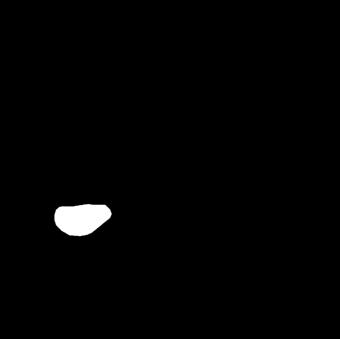
\includegraphics[width=0.85cm]{gt_mask.png}};
\node[font=\sffamily\tiny, below=0pt of gt] {mask};
\node[anchor=north west, align=left] at (14.4,1.5) {\textbf{A-clean}: drop defect patches\\from the mean (diagnostic)\\\textbf{A-median}, \textbf{A-trim}: no mask\\synthetic defects: 0.25--50\%};

\draw[arr] (12.75,3.4) -- (13.25,3.4);
\end{tikzpicture}
